%% 美赛模板:正文部分

\documentclass[12pt]{article}  % 官方要求字号不小于 12 号,此处选择 12 号字体

% 本模板不需要填写年份,以当前电脑时间自动生成
% 请在以下的方括号中填写队伍控制号
\usepackage[2009965]{easymcm}  % 载入 EasyMCM 模板文件
\problem{F}  % 请在此处填写题号
\usepackage{mathptmx}  % 这是 Times 字体,中规中矩 
%\usepackage{mathpazo}  % 这是 COMAP 官方杂志采用的更好看的 Palatino 字体,可替代以上的 mathptmx 宏包


\usepackage{rotating}
\usepackage{colortbl}
\usepackage{booktabs}
\usepackage{multicol}



\title{Arrangement for DroneGo}  % 标题

% 如需要修改题头(默认为 MCM/ICM),请使用以下命令(此处修改为 MCM)
%\renewcommand{\contest}{MCM}

% 文档开始
\begin{document}





% 此处填写摘要内容
\begin{abstract}

As global climate change continues, many island nations are threatened by rising sea levels. As a result, islanders face forced emigration. How to properly relocate these EDPs while ensuring the protection and preservation of their human rights and culture?This is what our team is trying to solve. To design the EDPs policy clearly, we divide the policy into the preservation policy of culture and the protection policy of human rights.

Our first model is the prediction model of potential EDPs. By using the sea level prediction model, we predicted the height of sea-level rise in 2100 (relative to 2000), and we selected 37 island countries at risk around the world based on the sea level rise in 2100 and the characteristics of the islands. We regard their citizens are all potential EDPs, and we estimated the number of potential EDPs. Next, we investigated the number of existing world heritage sites in these island countries and designed a series of preservation policies backed on the actual situation.

Our second model, from a human rights perspective, provides objective support for the design of EDPs' resettlement policies. Firstly, a Liveable Country Index (LCI) was created through the application of factor analysis to measure whether the host country can guarantee the human rights of EDPs. Similarly, the creation of a National Responsibility Index (NRI) to measure each country's responsibility for sea-level rise, namely each country's responsibility for the EDPs. Finally, considering the cost of migration distance, we created a Comprehensive Index from the perspective of risk island countries in different geographical locations, which represents the compatibility between island countries and host countries. We can see that the Comprehensive Index is the result of two-way selection.

According to the Composite Index, we have developed the best resettlement program under the premise of protecting human rights, for the EDPs. On this basis, some migration policies are put forward.At the end of the paper, we analyze the advantages and disadvantages of our model.


    % 美赛论文中无需注明关键字。若您一定要使用,
    % 请将以下两行的注释号 '%' 去除,以使其生效
     \vspace{5pt}
     \textbf{Keywords}: Sea-level Rise, EDPs , Migration Model, Factor Analysis.



\end{abstract}














\maketitle  % 生成 Summary Sheet
\tableofcontents  % 生成目录


% 正文开始
\section{Introduction}
\subsection{Background}



With the rising sea levels, the scene in the movie Waterworld is becoming a reality. Many island countries are disappearing at a rate that has exceeded most scientific forecasts. Some families and communities living on these island countries have already started to suffer from sea-level rise caused by climate change, which has forced them to leave their homes in search of a new beginning. Although the UN has acknowledged this issue and recognized that some EDPs might qualify as refugees, the international community still faces the problem of how to adequately settle EDPs based on protecting their human rights and culture.



%\begin{itemize}
%    \item Doing the first thing.
%    \item Doing the second thing.
%\end{itemize}

\subsection{Our work}
%A literatrue\cite{1} say something about this problem ...
To help the UN address the increasing challenge of EDPs, We need to develop a set of models for resettling policies that take into account the protection of human rights and the protection of culture. And we have done the following work: 

1. By predicting the future sea-level rise, estimate the potential EDPs and regions.

2. To analyze the risk of loss of the culture behind the EDPs. 

3. To guarantee the human rights of the EDPs, we established the evaluation models to arrange EDPs’ migration properly and provides  reference objectively 

4. According to the established model, our team designed the policies from two aspects: protecting human rights and protecting local culture.


%\begin{enumerate}[\bfseries 1.]
%    \item We do ...
%    \item We do ...
%    \item We do ...
%\end{enumerate}
\section{Assumptions}

\begin{itemize}
     \item  
     Population density does not change with time, which simplifies the process of calculating the population at risk.
     
     \item  
     Current national resources (e.g., arable land, freshwater) and GDP does not change over time,  to analyze the future migration policy of EDPs based on the current data.
     
     
     \item  
     The global mean sea level is used to estimate the risk area range, ignoring fluctuations in the sea surface caused by tides, waves, surges, or other disturbances.
\end{itemize}






\newpage
%----------------------------notations---------------------------

\section{Notations}
The primary notations used in this paper are listed in Table \ref{Notations}.
% Table generated by Excel2LaTeX from sheet 'Sheet1'
\begin{table}[htbp]
  \centering
  \caption{Notations}
    \begin{tabular}{ll}
    \toprule
    \multicolumn{1}{c}{Variable} & \multicolumn{1}{c}{Definition} \\
    \midrule
    $C(t)$  & Global emissions of greenhouse gases in year t \\
    
    $c_0$    & The initial CO$_2$ concentration(in 1850) \\
    $F(t)$  & radiative forcing in year t \\
    $a_0,b$  & \textcolor[rgb]{ .133,  .133,  .133}{Constant coefficient} \\
    $T(t)$  & \textcolor[rgb]{ .2,  .2,  .2}{Temperature in year t} \\
    $\beta$  & Specific heat capacity \\
    $\gamma$ & heat capacity ratio  \\
    $\kappa$ & \multicolumn{1}{p{25.555em}}{thermal diffusion coefficient of ocean} \\
    LCI   & Liveable Country Index \\
    NRI   & \textcolor[rgb]{ .133,  .133,  .133}{National Responsibility Index} \\
    IRI   & International Responsibility Index \\
    \toprule
    \end{tabular}%
  \label{Notations}%
\end{table}%



%4
\section{Preparation of Model}




%4.1
\subsection{Factor analysis}

\begin{itemize}

    \item Standardize the data obtained
    \begin{equation}
    X_i=\frac{X_i-E\left( X_i \right)}{\sqrt{Var\left( X_i \right)}}
\end{equation}


    
    \item Factor model
\begin{equation}
    \begin{cases}
	X_1=a_{11}F_1+a_{12}F_2+\cdots +a_{1m}F_m+\varepsilon _1\\
	X_2=a_{21}F_1+a_{22}F_2+\cdots +a_{2m}F_m+\varepsilon _2\\
	\,\,\vdots\\
	\,\,\vdots\\
	X_n=a_{n1}F_1+a_{n2}F_2+\cdots +a_{nm}F_m+\varepsilon _n\\
    \end{cases}
\end{equation}

It can also be expressed as:

\begin{equation}
    X=AF+\varepsilon 
\end{equation}

Where F is the factor variable, A is the factor load matrix, $a_{ij}$ is the factor load; $\epsilon$ is the special factor.





    \item Variance contribution rate (${k_i}$) of public factor $F_i$
    
    
    \begin{equation}
        k_i=\frac{\lambda _i}{\sum_{\gamma =1}^n{\lambda _{\gamma}}}\left( i=1,2...,n \right) 
    \end{equation}
    
    
$\lambda _i\left( \lambda _1,\lambda _2\cdots \cdots ,\lambda _n>0 \right) $
is the eigenvalue of the correlation coefficient matrix R of X.
    
    \item Factor load matrix
    \begin{equation}
            a_{ij}=\sqrt{\lambda _i}l_{ij}\left( i,j=1,2,...,n \right) 
    \end{equation}
    
    
    
\begin{equation}
    A=\left[ \begin{matrix}
	a_{11}&		\cdots&		a_{1m}\\
	\vdots&		\vdots&		\vdots\\
	a_{n1}&		\cdots&		a_{nm}\\
\end{matrix} \right] =\left[ \begin{matrix}
	\sqrt{\lambda _1}l_{11}&		\cdots&		\sqrt{\lambda _n}l_{n1}\\
	\vdots&		\vdots&		\vdots\\
	\sqrt{\lambda _1}l_{1n}&		\cdots&		\sqrt{\lambda _n}l_{nn}\\
\end{matrix} \right] 
\end{equation}

$I_{ij}$ is the correlation coefficient matrix R eigenvector.
    
    \item Factor variable score
    
    \begin{equation}
        F=AX
    \end{equation}

    \item Overall ratings
    
\begin{equation}
    Y_i=F_i\times k_i\,(i=1,2,…n)
\end{equation}

    
\end{itemize}











%5
\section{The Model for EDPs’ Number Valuation}

%5.1
\subsection{Prediction of sea level rise}

Carbon dioxide is the main cause of global sea level rise. We estimate future sea level rise by estimating carbon dioxide concentration.

%5.1.1
\subsubsection{Carbon dioxide concentration estimation}
According to the increase trend of future greenhouse gas emission and present research results, we assume the model of greenhouse gas emission is

\begin{equation}\label{ct}
    C\left( t \right) =c_0e^{Be^{at}}
\end{equation}







In order to make it convenient to estimate the parameters, we carry on the logarithm transformation to \eqref{ct}:



%公式2
\begin{equation}
    \ln C\left( t \right) =\ln c_0+B_te^{at}
\end{equation}


In this way, we only need to carry on simple least-squares estimate to model (2). Fitting with MATLAB to the emission data of global greenhouse gas since 1850, we obtain the following forecast model:

\begin{equation}
    \ln C(t)=-8.217+5.59\times 10^{-4}e^{8.70\times 10^{-3}t}\label{lnct}
\end{equation}



%5.1.2
\subsubsection{Greenhouse effect and temperature estimate}
In the role of the greenhouse conditions we assume that increase of greenhouse gas emissions is likely to cause an increase in the radiative forcing of the earth, the relationship between greenhouse gases and radiative forcing $F(t)$ is usually described by\eqref{ft}


\begin{equation}\label{ft}
    F\left( t \right) =a_0+b\ln \left[ c\left( t \right) /270 \right] 
\end{equation}


Where $a_0=1.81w/m^2$ and $b=2.95w/m^2$. $a_0$ and $b$ in the function can be adjusted appropriately according to the measured carbon dioxide emission concentration and the radiation intensity of the greenhouse effect.


Similarly, the temperature change caused by the emission of greenhouse gasses can be regarded as a function, which is obtained as the following:



\begin{equation}
    T\left( t \right) =\beta t\ln \left[ \gamma tC\left( t \right)\right]
\end{equation}


In equation, $\beta=0.00593$; $\gamma =0.0114$. According to scientists' estimates, the pre-industrial carbon dioxide emission concentration was $270\times10^{-6}$, and the temperature was about 0.68 degrees Celsius lower than that of 2000, which was considered zero in order to calculate sea-level changes.




%5.1.3
\subsubsection{Global sea level change prediction model}
In order to better link temperature changes, the greenhouse effect, and ocean thermal diffusion, we use the sea-level prediction equation from Wigley.

\begin{equation}
    Z\left( t \right) =\left[ 4.13+2.65F\left( t \right) \right] T\left( t \right) \kappa ^{0.221}
\end{equation}








$Z(t)$is the amount of sea-level rise or fall throughout time, the coefficient k is the value of thermal diffusion.

We take the values of k as 0.634, 1.2, 2.0, and 3.0, respectively. The estimated global sea-level rise trend is shown in Figure \ref{2000_2100} and sea level forecast for a particular year in Table \ref{Sea level forecast for a particular year}.



\begin{figure}[htbp]\label{2000_2100}
	\centering
	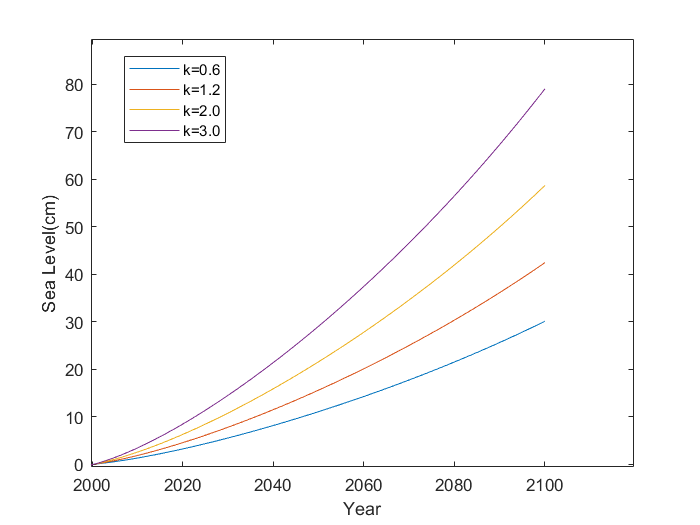
\includegraphics[width=.6\textwidth]{2000_2100.png}
	\caption{ The  estimated  global sea-level rise trend}\label{2000_2100}
\end{figure}


% Table generated by Excel2LaTeX from sheet 'Sheet2'
\begin{table}[htbp]
  \centering
  \caption{Sea level forecast for a particular year}
    \begin{tabular}{cccc}
    \toprule
    \multicolumn{1}{l}{\kappa} & 2030  & 2050  & 2100 \\
    \midrule
    0.6   & 5.5(cm)   & 11.1(cm)  & 30.1(cm) \\
    1.2   & 7.8   & 15.6  & 42.4 \\
    2     & 10.8  & 21.6  & 58.6 \\
    3     & 14.5  & 29    & 78.9 \\
    \bottomrule
    \end{tabular}%
  \label{Sea level forecast for a particular year}%
\end{table}%





The difference between the model and the real data(data source: NASA) is shown in Figure \ref{2000_2010}. We use mean square error (MSE) to compare the differences between the 4 models and the real data. The MSE values of the four models are 4.78, 2.29, 0.43, 0.38 respectively. When $\kappa = 3$, the model fits best.



\begin{figure}[htbp]
	\centering
	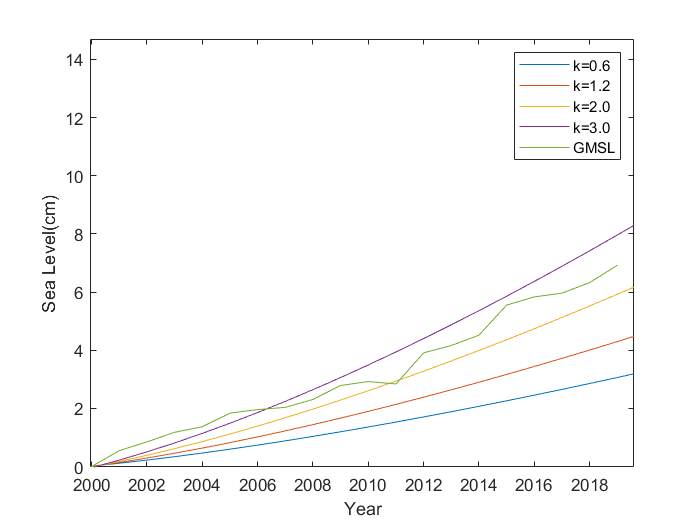
\includegraphics[width=.6\textwidth]{2000_2010.png}
	\caption{ The difference between the model and the real data}\label{2000_2010}
\end{figure}






%5.2
\subsection{The Risky Area and Population}

It can be seen from the above prediction that sea level will rise by 78.9cm in 2100 relative to 2000. This rise will result in the inundation and salinization of large areas of land in many coastal areas and islands. Then the land becomes uninhabitable, and the people who lived on it must move to other lands. For coastal countries with large landmasses, their at-risk populations will naturally migrate within their borders without creating environmental refugees. 

By contrast, island nations have no more room to accommodate their citizens who have lost their homes because of rising seas, so we can consider they are potential environmental refugees.
 For different types of island nations, however, the effects of rising sea levels on land flooding and salinization are different. Over this century, large swathes of island countries (such as Japan and Britain) will have plenty of land to house their at-risk populations. On the contrary, for small island countries, because the whole country is in the risk zone, there are a large number of potential environmental refugees.
 
Across the globe, we have picked out island countries smaller than 30,000km$^2$ and identified their inhabitants as potential environmental refugees. 
A total of 37 island states are threatened (see appendix for details) with a current population of 30,460,103. The geographical location is shown below.


\begin{figure}[htbp]\label{5.2}
	\centering
	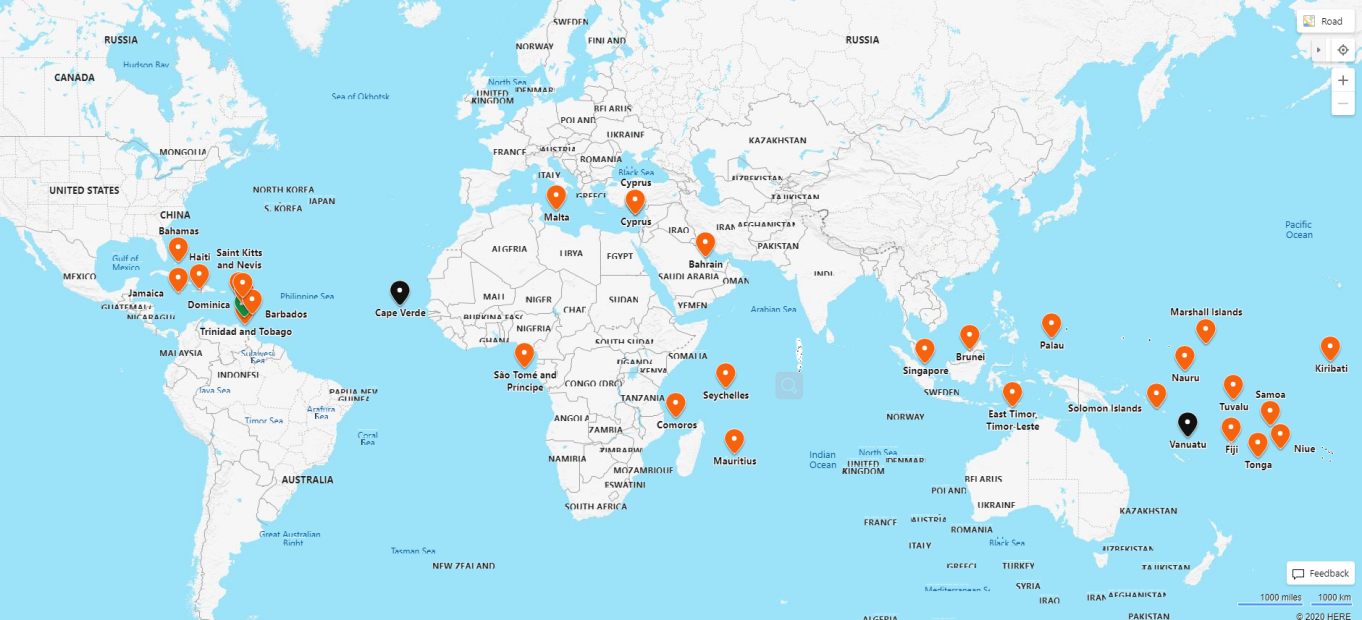
\includegraphics[width=1\textwidth]{5.2.png}
	\caption{ The geographical locations of 37 island states}\label{5.2}
\end{figure}



\newpage
%6
\section{Preservation of Culture Policy}

%6.1
\subsection{The risk of loss of culture}
Statistics show that there are 27 world heritage sites scattered among the 37 risk island countries.These world heritage sites are divided into Cultural site and Natural site.From figure \ref{culture site}, we can see that about 70\% are cultural sites, about 22\% are natural cultural heritage, and another 7\% are in extreme danger.They are of high cultural value.(see appendix for details of world heritage).

\begin{figure}[htbp]
	\centering
	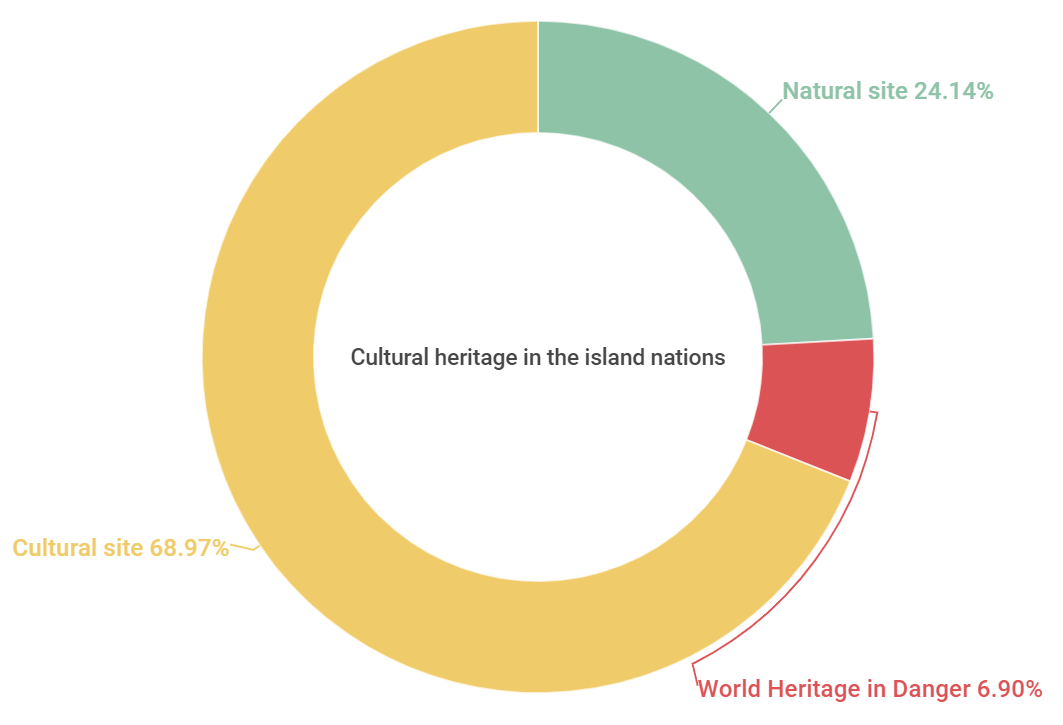
\includegraphics[width=.8\textwidth]{culture site.png}
	\caption{ World Heritage}\label{culture site}
\end{figure}

There is an urgent need to protect the vast number of world cultural heritage sites that are scattered among these at-risk island countries.A series of protection policies is very necessary.



%6.2
\subsection{Concrete Policies}
Our team has divided cultural protection into three levels , as shown in figure \ref{culture 3 levels}, and proposed corresponding policies.

\begin{figure}[htbp]
	\centering
	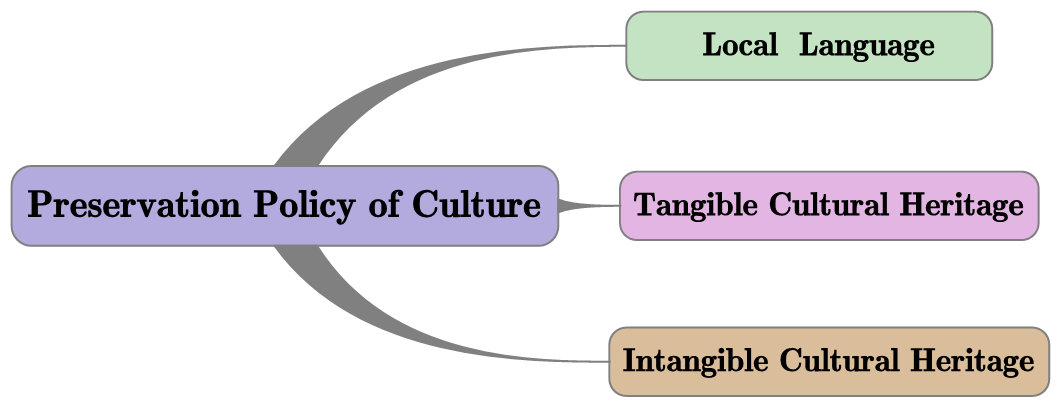
\includegraphics[width=.8\textwidth]{culture 3 levels.png}
	\caption{ Three levels of culture protection }\label{culture 3 levels}
\end{figure}


%6.2.1
\subsubsection{Local Language}
Language can reflect the world outlook, the way of thinking, social characteristics, and culture of the user's nation. The main reason for the demise of languages is that society is moving towards more politically and economically dominant languages. Generally speaking, the language of the host country is more influential than the minor languages of the EDPs country, so it is necessary to protect the minor languages used by EDPs after they migrate to host countries.



(1)\textbf{Establish multimedia language corpus.} Records the unique languages, dialects, and spoken words of island countries, processed into a language resource database. The protection of local languages should begin before large numbers of EDPs leave the country. The support of linguists and local governments is also needed, as are the policy and financial supports of the international community.


(2)\textbf{Set up island language learning institutions.} Establish some island language learning institutions in selected recipient countries. This policy can stimulate the interest of the host country's people in the language and culture of EDPs. It helps to protect the language and culture of EDPs, and at the same time, reduces the conflict between the two peoples, making it easier for EDPs to integrate into the host country.



(3)\textbf{Select coastal countries as host countries.} The EDPs come from almost the tropical island countries that are surrounded by the sea. The choice of littoral states as host country is conducive to the rapid adaptation of EDPs to life after migration and the continuation of the culture of these island countries.





%6.2.2
\subsubsection{Intangible Cultural Heritage}

(1)\textbf{Promote the intangible cultural heritage of at-risk island countries.}Through the media and other means to actively spread and increase external publicity, this can not only increase the residents' understanding of the culture of the EDPs but also reduce the cultural conflicts between residents and EDPs in the host countries. At the same time, museums should be set up actively, which can not only protect the tangible cultural heritage but also transform the intangible cultural heritage into videos, pictures, and other media.


(2)\textbf{The host country should make laws and regulations to protect EDPs.} A large number of refugees from the host country may lead to cultural conflicts such as customs and languages between the EDPs and the original residents. The host country should make similar laws and regulations to protect the culture of refugees and avoid discrimination against EDPs by residents.







%6.2.3
\subsubsection{Tangible Cultural Heritage}

(1)\textbf{Build museums to preserve the unique cultural relics.} The governments of EDPs countries should actively excavate and preserve local cultural relics and, in cooperation with the host countries, establish museums in the host countries in advance to display and protect their unique historical relics.



(2)\textbf{Establish an expert group to design plans for the removal of cultural sites.} Many of the cultural heritage sites of at-risk island nations are under threat, with many of them likely to be submerged as sea levels rise. Cultural sites should be relocated as soon as possible, or we have to prepare for marine protection. 




%7
\section{The Model for EDPs’ Migration}

%7.1
\subsection{Liveable Country Index (LCI)}
A person cannot survive without land, property, freshwater, and food. The premise for a country to accept EDPs is to guarantee fundamental human rights, such as the right to life, land, work, and freshwater. So we selected population density, per capita GDP, per capita freshwater resources, and per capita arable land as indicators to measure the country's settable index. The higher the Liveable Country Index, the better the country can guarantee the human rights of EDPs.

Then we calculated the Liveable Country Index of each country(not include island countries) through the factor analysis method in the SPSS software based on the collected data and selected the country with the LCI greater than 0 as the country suitable for accepting EDPs. The result is shown in figure \ref{Countries_with_eligible_immigration_indices}.

\begin{figure}[htbp]
	\centering
	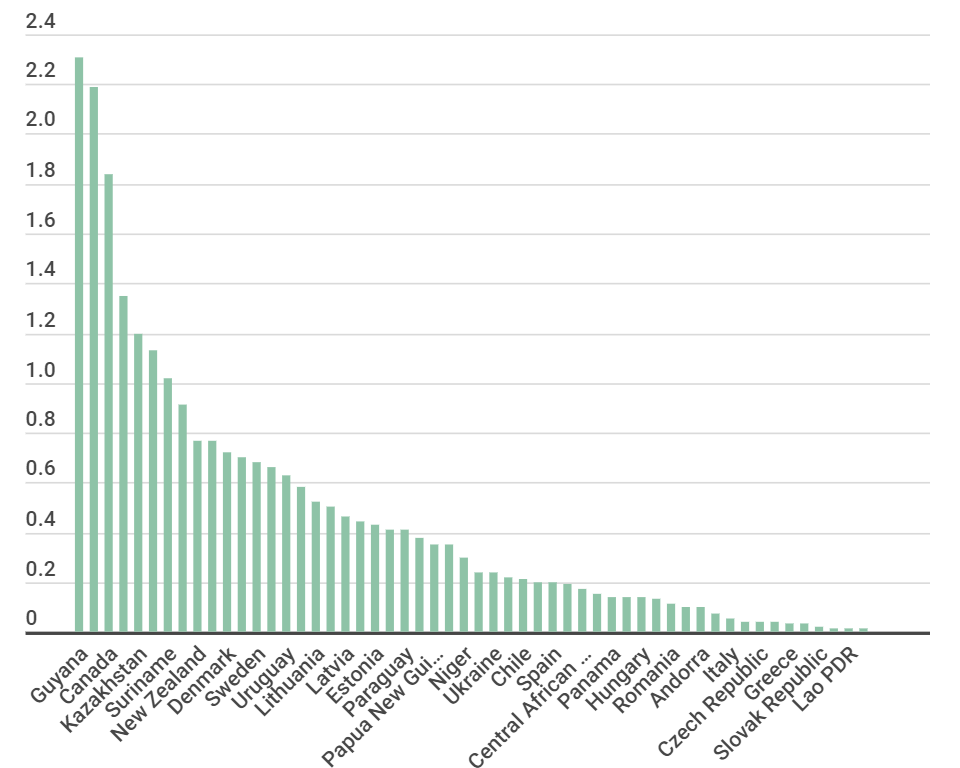
\includegraphics[width=.8\textwidth]{LCI.png}
	\caption{ Countries with the LCI greater than 0 }
	\label{Countries_with_eligible_immigration_indices}
\end{figure}





%7.2
\subsection{National Responsibility Index (NRI)}
First, we select per capita CO$_2$ emissions and per capita energy consumption as indicators of the National Responsibility Index, because the greenhouse effect is the leading cause of sea-level rise. The higher the National Responsibility Index, the more responsible a country is to accept EDPs.


After that, we normalize per capita CO$_2$ emissionss and per capita energy consumption of countries with LCI value greater than 0, and measure their contribution to the National Responsibility Index with a weighting of 50\% each. The corresponding NRI of 57 countries was obtained. The results are shown in figure \ref{NRI}.

\newpage
\begin{figure}[htbp]
	\centering
	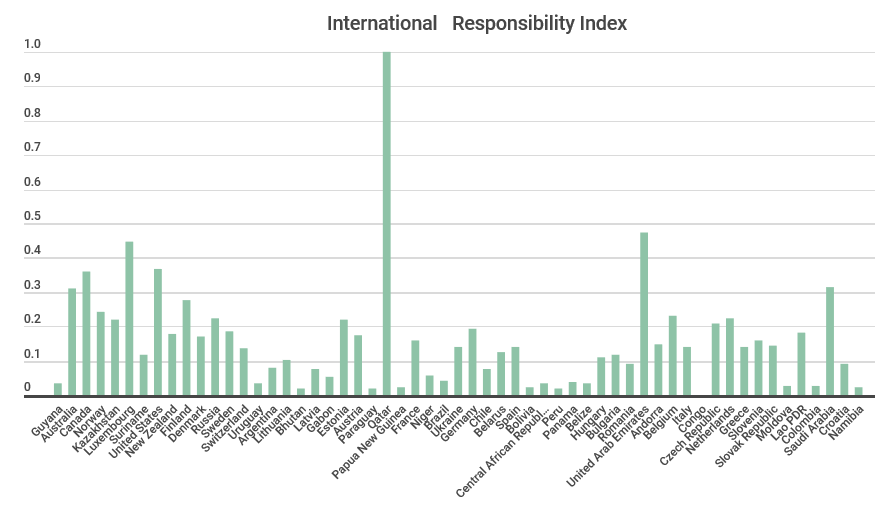
\includegraphics[width=.8\textwidth]{NRI.png}
	\caption{ The NRI of 57 countries}\label{NRI}
\end{figure}










%7.3
\subsection{International Responsibility Index (IRI)}

When policymakers consider which countries should accept displaced refugees, they should not only consider whether the country has a pleasant living environment or how much it contributes to global warming. They should combine the two to get more objective results. Therefore, we merged LCI and NRI into the International Responsibility Index. Countries with high IRI should give priority to accept EDPs.

The migration index of selected countries was normalized, and the contribution to IRI was measured by weighting LCI and national NRI at 50\% each.


\begin{equation}\label{IRI}
    IRI=0.5\times normalized\,\,LCI+0.5\times NRI
\end{equation}


Through equation \eqref{IRI}, the IRI of 57 countries are shown in figure. \ref{country_index}

\begin{figure}[htbp]
	\centering
	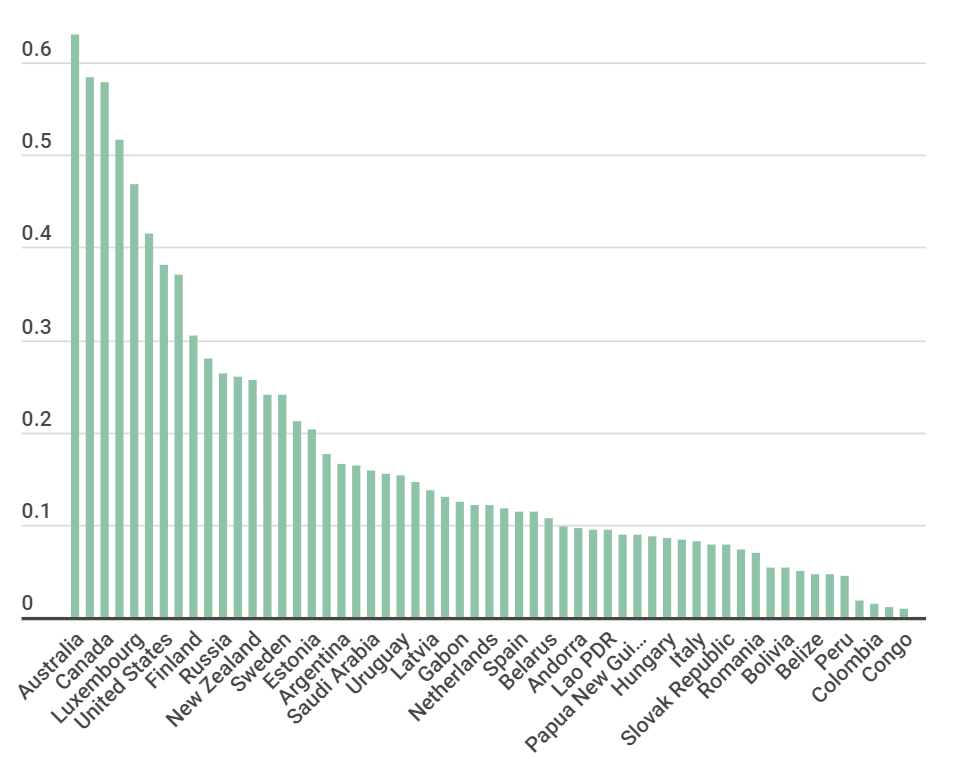
\includegraphics[width=.8\textwidth]{IRI.png}
	\caption{ The IRI of 57 countries}\label{country_index}
\end{figure}

\newpage



%-----------------------------------high index countries-----------------------
We regard countries with an IRI greater than 0.3 to be high. To simplify the subsequent calculations, we used only high-index countries. The result is shown in figure \ref{high_index_countries}.



\begin{figure}[htbp]
	\centering
	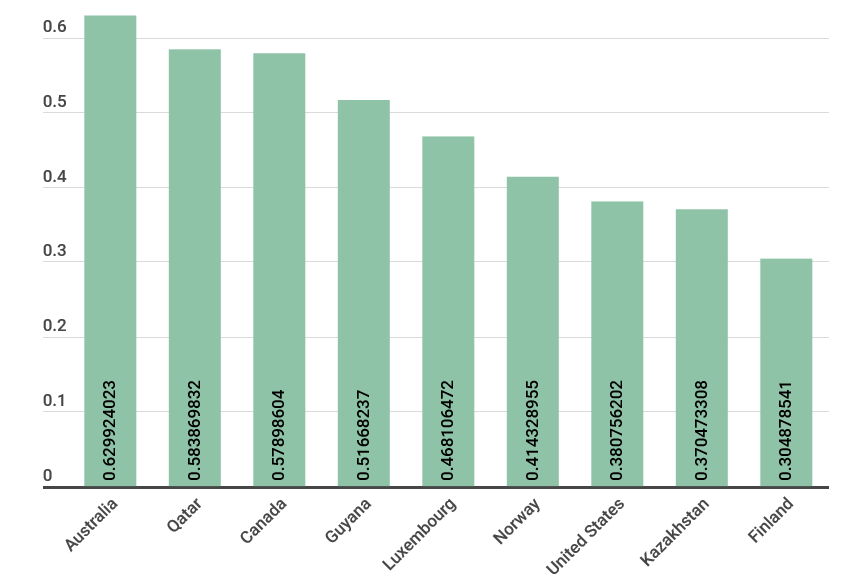
\includegraphics[width=.8\textwidth]{high_index_countries.png}
	\caption{Countries with an IRI greater than 0.3}\label{high_index_countries}
\end{figure}





%7.4
\subsection{The influence of geographical distance on resettlement}

The island nations at risk are scattered across the world's oceans. Long-distance migration is not only expensive but also inefficient; thus, the influence of geography on resettlement must be taken into account when considering the problem of EDPs. Therefore, we regard the distance between island countries and countries with high IRI as one of the factors determining our policy.



Based on geographical location, we divided the 37 threatened countries into six regions: Caribbean Sea(A), Western Pacific(B), Mediterranean Sea(C), Maritime Southeast Asia(D), Indian Ocean(E), East Atlantic(F). The countries included in each region are shown in figure \ref{6_regions}.


\begin{figure}[htbp]
	\centering
	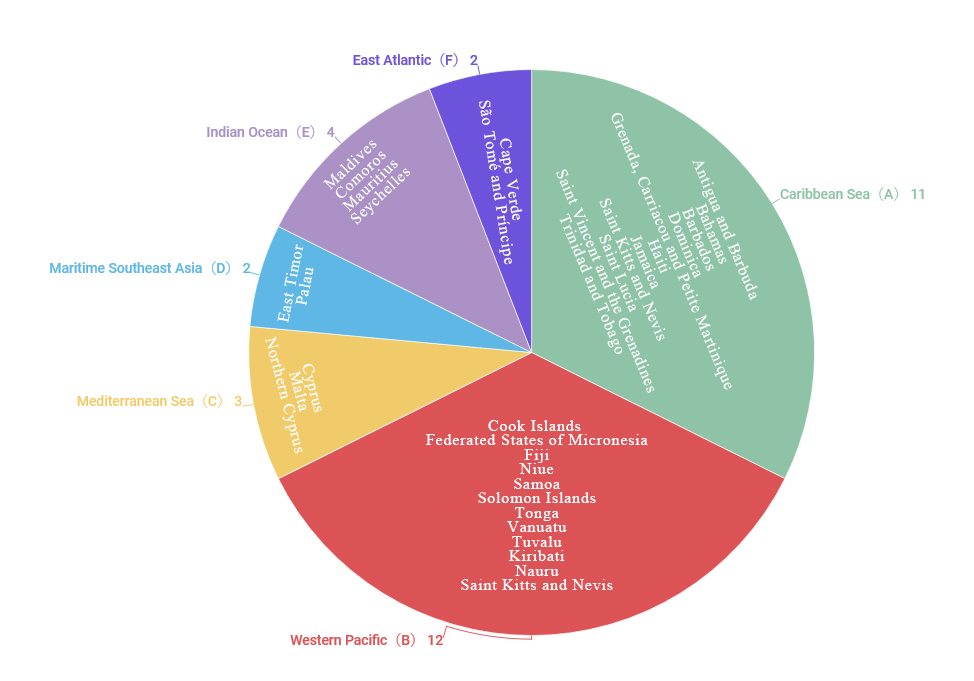
\includegraphics[width=.8\textwidth]{6_regions.png}
	\caption{ 6 regions}\label{6_regions}
\end{figure}




Bing Map was used to measure the distance between countries with high country index and threatened areas, and the distance was divided into 6 grades, as shown in Table \ref{distance_level}.



% Table generated by Excel2LaTeX from sheet 'Sheet1'
\begin{table}[htbp]
  \centering
  \caption{Add caption}
    \begin{tabular}{lllllll}
    \toprule
    Rank  & \multicolumn{1}{c}{1} & \multicolumn{1}{c}{2} & \multicolumn{1}{c}{3} & \multicolumn{1}{c}{4} & \multicolumn{1}{c}{5} & \multicolumn{1}{c}{6} \\
    \midrule
    Distance(km) & <3000 & 3000-6000 & 6001-9000 & 9001-12000 & 12001-15000 & 15001-18000 \\
    \bottomrule
    \end{tabular}%
  \label{distance_level}%
\end{table}%



After the measurement, we got table \ref{distance}.



% Table generated by Excel2LaTeX from sheet 'Sheet1'
\begin{table}[htbp]
  \centering
  \caption{Add caption}
    \begin{tabular}{lcccccc}
    \toprule
    Country & A     & B     & C     & D     & E     & F \\
    \midrule
    Australia & 6     & 2     & 5     & 1     & 4     & 6 \\
    Qatar & 4     & 5     & 2     & 3     & 2     & 3 \\
    Canada & 2     & 4     & 3     & 5     & 5     & 5 \\
    Guyana & 1     & 5     & 3     & 6     & 4     & 3 \\
    Luxembourg & 3     & 6     & 1     & 5     & 3     & 2 \\
    Norway & 3     & 5     & 2     & 4     & 3     & 3 \\
    United States & 1     & 4     & 3     & 6     & 5     & 3 \\
    Kazakhstan & 4     & 4     & 2     & 3     & 3     & 3 \\
    Finland & 3     & 5     & 2     & 4     & 3     & 3 \\
    \bottomrule
    \end{tabular}%
  \label{distance}%
\end{table}%





%7.5
\subsection{Comprehensive Index}
For more careful consideration, IRI and distance grade was used as the comprehensive indexes to select suitable countries for EDPs to resettle. Closer proximity means lower resettlement costs and, to some extent, it protect EDPs' way of life. The evaluation system of the comprehensive index was defined as:

\begin{equation}
    Comprehensive\,\,Index=IRI-\frac{Distance\,\,grade}{Maximum\,\,Distance\,\,grade}+0.6
\end{equation}


The 0.6 here is to prevent the composite index from being negative, which would affect the comparison between the results.

\begin{figure}[htbp]
	\centering
	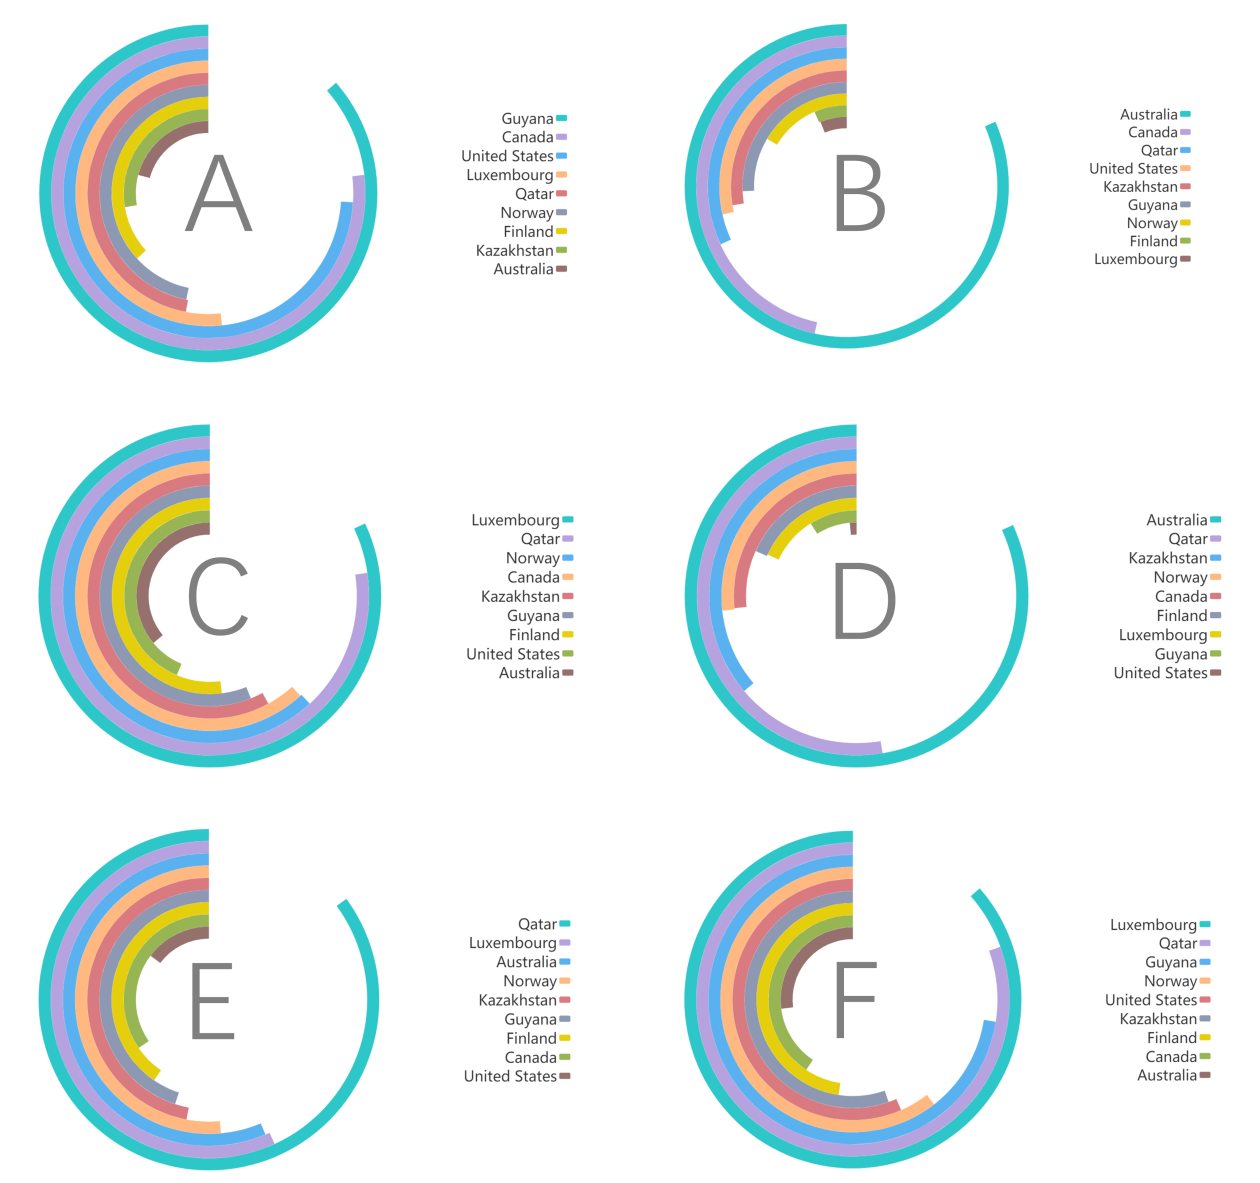
\includegraphics[width=.8\textwidth]{ABCDEF.png}
	\caption{ flow diagram of solution}\label{ABCDEF}
\end{figure}


\newpage

%-------------------------------------8
\section{Migration Policy Based on Protection of Human Rights}
With the support of the above model, we developed an immigration policy that fully protects the EDPs' human rights, as shown below:



1. \textbf{UN should make accurate statistics of country data for calculation of the Comprehensive Index}, for the island countries in different geographical locations to choose the suitable host country. The Composite Index of island countries in one of six sea regions varies with different host countries. Depending on the difference in the Composite Index, host countries may accept the EDPs from the same sea region in proportion to the Composite Index. This would be fairer to the host countries and would not result in a large number of EDPs crowding in one host country.




2. \textbf{Establish a special international relief fund for climate refugees}. The money should come from developed countries that are mainly responsible for climate change, with some earmarked for climate refugees. The division of responsibility is demanding. So we determine each country's "national responsibility index" based on its CO2 emissions and per capita energy consumption. The larger the index, the higher the country's responsibility for global climate change, to determine which countries are obliged to participate in the financing and the proportion of financing.






%-------------------------------------9
\section{Strengths and Weaknesses}



%9.1
\subsection{Strengths}

\textbf{The first model}: This paper roughly estimated the potential population of EDPs based on the prediction of sea-level rise. Meanwhile, we analyzed the risk of cultural loss of EDPs and established a series of models. On the basis of these models, we proposed sets of the proposed policy to deal with EDPs in terms of human rights and  preservation of unique island culture.


\textbf{Second model}: Although the EDPs in different situations, the Conprehensive Index can be used to provide the optimal solution for the host country. At the same time, the ability of the host country to accept EDPs is fully considered, so that EDPs can be well integrated into the host country and will not become a burden on the host country. The most important thing is to properly balance the human rights of the EDPs with the responsibilities of the host country.





%9.2
\subsection{Weaknesses}

\textbf{The first model}: Ignoring the elevation of an island country and using its area as an indicator of whether an island country is at risk, it will lead to inaccurate estimates of the potential EDPs population.




\textbf{The second model}: due to limited space and time, not enough factors were considered in the evaluation of LCI and IRI.In the subsequent use of the model, new influencing factors can be taken in to improve the model.




%%%%%%%%%%%%%%%%%%%%%%%%%%%%%%%%%%%%%%%%%%%%%%%%%%%%%%%%%%%%%%%%%%%%

% 参考文献,此处以 MLA 引用格式为例
\begin{thebibliography}{99}
\bibitem{1} Einstein, A., Podolsky, B., \& Rosen, N. (1935). Can quantum-mechanical description of physical reality be considered complete?. \emph{Physical review}, 47(10), 777.
\bibitem{2} \emph{A simple, easy \LaTeX\ template for MCM/ICM: EasyMCM}. (2018). Retrieved December 1, 2019, from\url{https://www.cnblogs.com/xjtu-blacksmith/p/easymcm.html}


\bibitem{3} Wigley, T., Schlesinger, M. Analytical solution for the effect of increasing CO$_2$ on global mean temperature. \emph{Nature} 315, 649–652 (1985). \url{https://doi.org/10.1038/315649a0}





\end{thebibliography}
%%%%%%%%%%%%%%%%%%%%%%%%%%%%%%%%%%%%%%%%%%%%%%%%%%%%%%%%%%%%%%%%%%%%%





% 如您的论文中不需要附录,请自行删除
\begin{subappendices}  % 附录环境

\section{Appendix A: Further on \LaTeX}
To clarify the importance of using \LaTeX\ in MCM or ICM, several points need to be covered, which are \ldots

To be more specific, \ldots

All in all, \ldots

Anyway, nobody \textbf{really} needs such appendix \ldots

\end{subappendices}



%%%%%%%%%%%%%%%%%%%%%%%%%%%%%%%%%%%%%%%%%%%%%%%%%%%%%%%%%%%%%%%%%%%%%%%%%


\section{XXXXXXXXXXXXXXXXXXXXXXXXXXXXXXXXXXXXXX}

Above all, in terms of the number of containers, it is obvious that more containers can provide more drones and medical supply. 

In addition, the area where the phrasecontainer is located can charge the drones. 
	
	Therefore, more containers will makethe drones more flexible and create a wider reconnaissance range. The most important point is that one or two cargo containers cannot cover the five hospitals(this will be shown in Part 7). Due to the reasons above, we firstly consider the
	number of containers is 3.
	
	We think the helicopter has the ability to transport containers to inland. Therefore, in terms of the location of the container, we need to consider the location of the container inside Puerto Rico so that the container can meet the daily needs of
	the hospital and the road reconnaissance.


\begin{table}[htbp]
	\centering
	\caption{Sea level prediction at a specific time}
	\begin{tabular}{c|ccc}
		\toprule
		\kappa     & 2030  & 2050  & 2100 \\
		\midrule
		0.634 & 9.45  & 15.48 & 32.28 \\
		1.2   & 10.89 & 17.82 & 37.16 \\
		2     & 12.19 & 19.95 & 41.6 \\
		3     & 13.3  & 21.83 & 45.5 \\
		\bottomrule
	\end{tabular}%
	\label{tab:addlabel}%
\end{table}%





%The detail can be described by equation \eqref{eq:heat}:
%\begin{equation}\label{eq:heat}
%\frac{\partial u}{\partial t} - a^2 \left( \frac{\partial^2 u}{\partial x^2} + \frac{\partial^2 u}{\partial y^2} + \frac{\partial^2 u}{\partial z^2} \right) = f(x, y, z, t)
%\end{equation}
\begin{figure}[htbp]
	\centering
	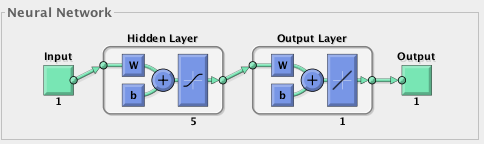
\includegraphics[width=.6\textwidth]{p1.png}
	\caption{ flow diagram of solution}\label{fig: flow diagram of solution}
\end{figure}



\subsection{Model 2}
The results are shown in Figure \ref{fig: flow diagram of solution}, where $t$ denotes the time in seconds, and $c$ refers to the concentration of water in the boiler.

\begin{figure}[htbp]
\centering
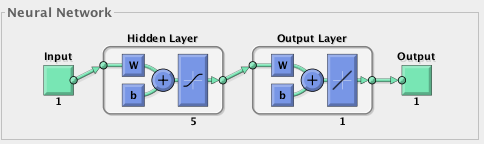
\includegraphics[width=.6\textwidth]{p1.png}
\caption{ flow diagram of solution}\label{fig: flow diagram of solution}
\end{figure}
We get the following equation\eqref{eq:complex}
\begin{equation}\label{eq:complex}
		T=\frac{D\times    V_m}{\sum_{i=1}^{n_d}{\frac{z_i}{\frac{d_i}{v_i+T_0}}}}
\end{equation}
\newpage
\section{Strengths and Weaknesses}
\subsection{Strengths}
\begin{itemize}
    \item First one...
    \item Second one ...
\end{itemize}
\begin{figure}[htbp]
	\begin{minipage}{0.45\linewidth}
		\centering
		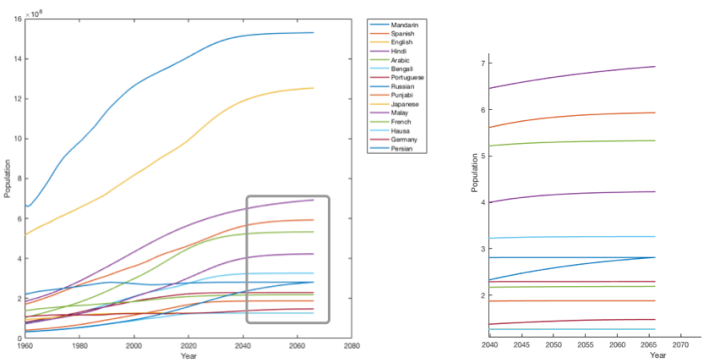
\includegraphics[width=\textwidth]{p3.png}
		\caption{Geometrical relationship} 
		\label{fig:beta}
	\end{minipage}
	\begin{minipage}{0.45\linewidth}
		\centering
		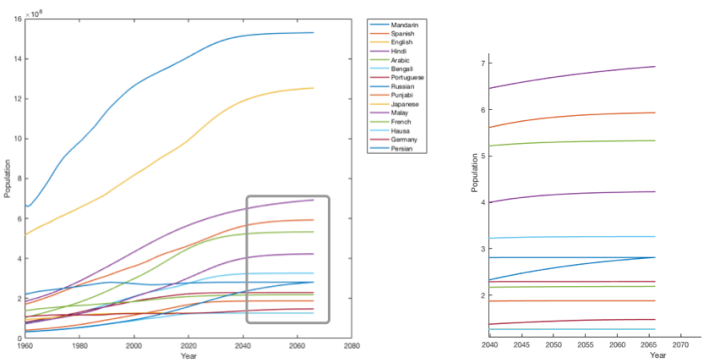
\includegraphics[width=\textwidth]{p3.png}
		\caption{The $F_s$ under ND control}
		\label{fig:Force_plane}
	\end{minipage}
\end{figure} 

\subsection{Weaknesses}
\begin{itemize}
    \item Only one ...
 \end{itemize}


% 以下为信件/备忘录部分,不需要可自行去掉
% 如有需要可将整个 letter 环境移动到文章开头或中间
% 请在后一个花括号内填写信件(Letter)或备忘录(Memorandum)标题
\begin{letter}{Memorandum}
\begin{flushleft}  % 左对齐环境,无首行缩进
\textbf{To:} Heishan Yan\\
\textbf{From:} Team XXXXXXX\\
\textbf{Date:} October 1st, 2019\\
\textbf{Subject:} A better choice than MS Word: \LaTeX
\end{flushleft}

In the memo, we want to introduce you an alternate typesetting program to the prevailing MS Word: \textbf{\LaTeX}. In fact, the history of \LaTeX\ is even longer than that of MS Word. In 1970s, the famous computer scientist Donald Knuth first came out with a typesetting program, which named \TeX\ \ldots

Firstly, \ldots

Secondly, \ldots

Lastly, \ldots

According to all those mentioned above, it is really worth to have a try on \LaTeX! 
\end{letter}


% 参考文献,此处以 MLA 引用格式为例
\begin{thebibliography}{99}
\bibitem{1} Einstein, A., Podolsky, B., \& Rosen, N. (1935). Can quantum-mechanical description of physical reality be considered complete?. \emph{Physical review}, 47(10), 777.
\bibitem{2} \emph{A simple, easy \LaTeX\ template for MCM/ICM: EasyMCM}. (2018). Retrieved December 1, 2019, from\url{https://www.cnblogs.com/xjtu-blacksmith/p/easymcm.html}
\end{thebibliography}


% 以下为附录内容

\end{document}